\documentclass{beamer}
\usetheme{Boadilla}

\usepackage{amsmath}
\usepackage{amsfonts}
\usepackage{hyperref}
\usepackage{xcolor}

\usepackage{amsmath}
\DeclareMathOperator*{\argmax}{arg\,max}
\DeclareMathOperator*{\argmin}{arg\,min}

\title{Variational Mixture-of-Experts Autoencoders for Multi-Modal Deep Generative Models}
\author{Kseniia Petrushina}
\institute{MIPT, 2023}


\begin{document}

\begin{frame}
    \titlepage
\end{frame}


\begin{frame}
    \tableofcontents
\end{frame}


\section{Motivation \& Background}
\begin{frame}{Motivation}
    \begin{figure}
        \centering
        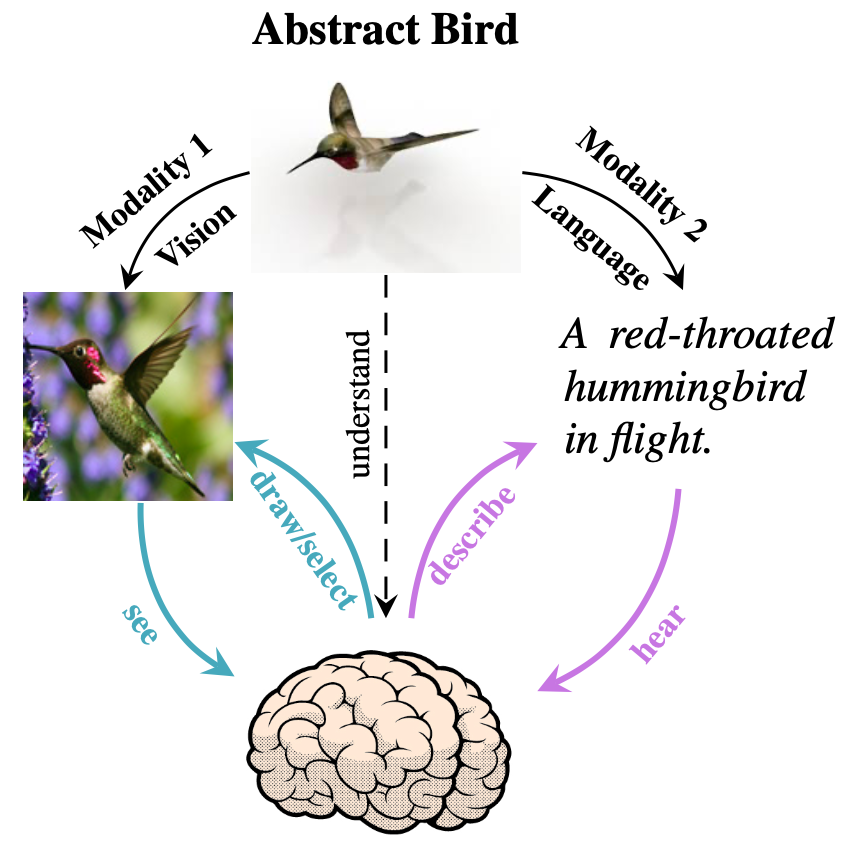
\includegraphics[scale=0.2]{brain.png}
        \caption{A schematic for multi-modal perception.}
        \label{fig:brain}
    \end{figure}
\end{frame}

\begin{frame}{Motivation}
    \begin{figure}
        \centering
        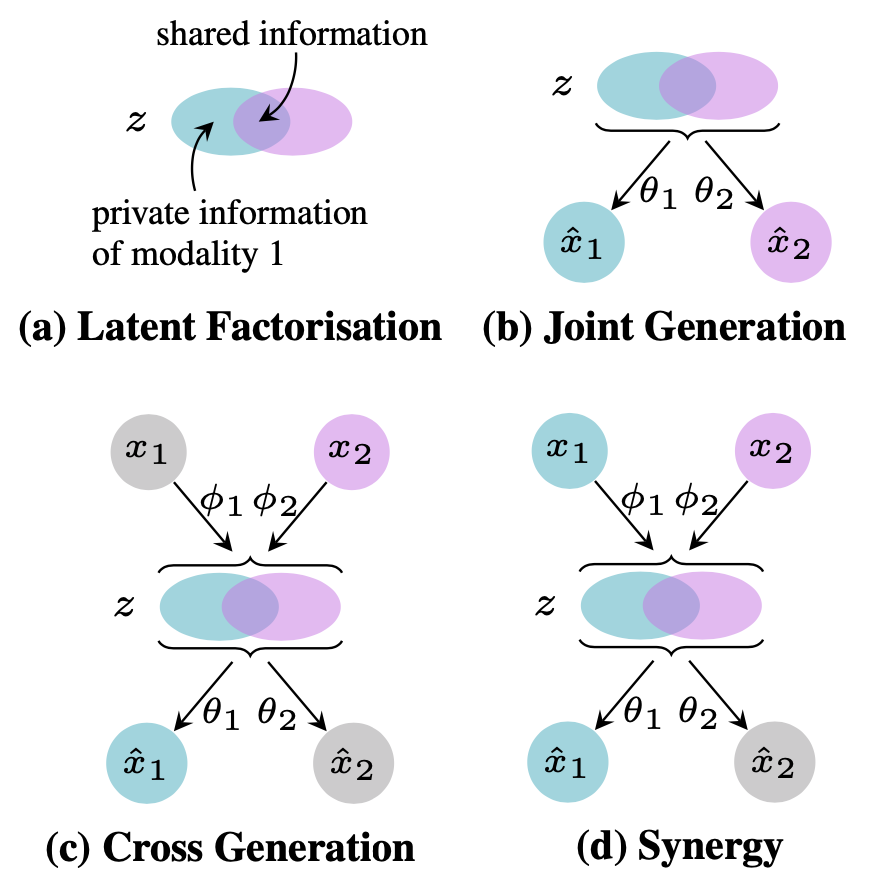
\includegraphics[scale=0.2]{criteria.png}
        \caption{The four criteria for multi-modal generation models.}
        \label{fig:criteria}
    \end{figure}
\end{frame}


\begin{frame}{Background}
 \begin{block}{VAE}
    \textbf{Goal}: $$p_\Theta(\textbf{z}, \textbf{x}_{1, \dots, M}) = p(\textbf{z})\prod\limits_{m=1}^M p_{\theta_m}(\textbf{x}_m | \textbf{z})$$

    \textbf{Training objective}: $$p_\Theta (\textbf{x}_{1:M}) \to \max\limits_\Theta$$

    True posterior $ p_\Theta(\textbf{z}| \textbf{x}_{1: M}) \to $ variational posterior $q_\Phi(\textbf{z}| \textbf{x}_{1: M})$
    
\end{block}
    
\begin{block}{ELBO}

    $$\mathcal{L}_\text{ELBO}(\textbf{x}_{1:M}) = \mathbb{E}_{\textbf{z}\sim q_\Phi (\textbf{z}| \textbf{x}_{1: M})} \Bigl[ \log \dfrac{p_\Theta(\textbf{z}, \textbf{x}_{1:M})}{q_\Phi (\textbf{z} | \textbf{x}_{1:M})} \Bigr]$$

    $$\mathcal{L}_\text{IWAE}(\textbf{x}_{1:M}) = \mathbb{E}_{\textbf{z}^{1:K}\sim q_\Phi (\textbf{z} | \textbf{x}_{1: M})} \Bigl[ \log \sum\limits_{k=1}^K \dfrac1K \dfrac{p_\Theta(\textbf{z}^k, \textbf{x}_{1:M})}{q_\Phi (\textbf{z}^k | \textbf{x}_{1:M})} \Bigr] $$
\end{block}
\end{frame}

\begin{frame}{Joint variational posterior}
 \begin{block}{Product of experts}
    $$q_\Phi (\textbf{z}| \textbf{x}_{1:M}) = \prod\limits_{m=1}^M q_{\phi_m} m(\textbf{z}| \textbf{x}_m)$$

    \begin{itemize}
        \item[-] Low total density if one of the the factors has low density -- each expert has veto power
        \item[-] Overconfidence in predictions has detrimental consequences for the model
    \end{itemize}
    
\end{block}

\begin{block}{Mixture of experts}
    $$q_\Phi(\textbf{z}| \textbf{x}_{1:M}) = \dfrac1M \sum\limits_{m=1}^M q_{\phi_m} (\textbf{z}| \textbf{x}_m)$$

\end{block}

\end{frame}

\section{Theory}
\begin{frame}{MoE-multimodal VAE}
    \begin{block}{Objective}
    $$\mathcal{L}_\text{IWAE}^\text{MoE} (\textbf{x}_{1:M}) = \dfrac1M \sum\limits_{m=1}^M \mathbb{E}_{\textbf{z}^{1:K}_m \sim q_{\phi_m} (\textbf{z} | \textbf{x}_{m})} \Bigl[ \log \dfrac1K  \sum\limits_{k=1}^K \dfrac{p_\Theta(\textbf{z}^k_m, \textbf{x}_{1:M})}{q_\Phi (\textbf{z}^k_m | \textbf{x}_{1:M})} \Bigr] $$

    \end{block}    

    \begin{block}{Theorem}

    $$\mathcal{L}_\text{ELBO} (\textbf{x}_{1:M}) \le \mathcal{L}_\text{IWAE}^\text{MoE} (\textbf{x}_{1:M})$$
    
    \end{block}

    \begin{block}{Proof}
    $$\mathcal{L}_\text{ELBO} (\textbf{x}_{1:M}) = \mathbb{E}_{\textbf{z}\sim q_\Phi (\textbf{z}| \textbf{x}_{1: M})} \Bigl[ \log \dfrac{p_\Theta(\textbf{z}, \textbf{x}_{1:M})}{q_\Phi (\textbf{z} | \textbf{x}_{1:M})} \Bigr] =  $$ $$=\dfrac1M \sum\limits_{m=1}^M \mathbb{E}_{\textbf{z}_m \sim q_{\phi_m} (\textbf{z}| \textbf{x}_{m})} \Bigl[ \log \dfrac{p_\Theta(\textbf{z}_m, \textbf{x}_{1:M})}{q_\Phi (\textbf{z}_m | \textbf{x}_{1:M})} \Bigr] \le \mathcal{L}_\text{IWAE}^\text{MoE} (\textbf{x}_{1:M})$$

    \end{block}
    
\end{frame}


\section{Empirical results}
\begin{frame}{MNIST-SVHN}
    \begin{figure}
        \centering
        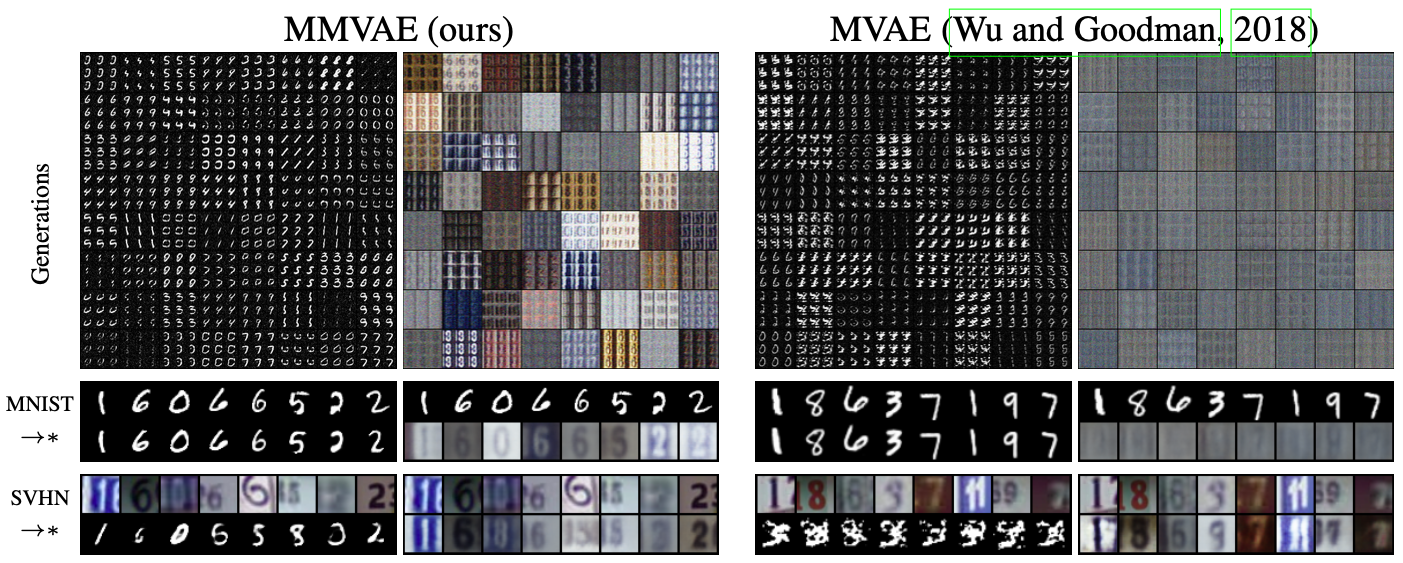
\includegraphics[scale=0.24]{qual.png}
        \caption{Qualitative results on MNIST-SVHN dataset pair.}
        \label{fig:qual}
    \end{figure}
\end{frame}

\begin{frame}{MNIST-SVHN}
    \begin{figure}
        \centering
        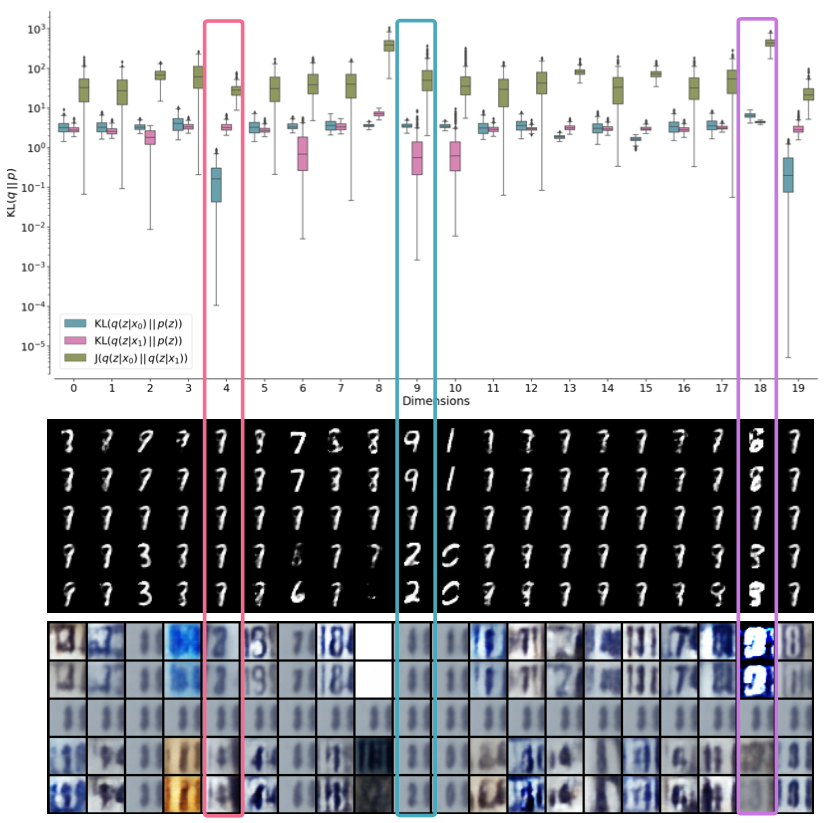
\includegraphics[scale=0.2]{latent.png}
        \caption{Per-dimension latent traversals for a pair of datapoints indicating dimensions that affect only \textcolor{magenta}{SVHN}, only \textcolor{cyan}{MNIST}, and both \textcolor{violet}{MNIST \& SVHN}.}
        \label{fig:latent}
    \end{figure}
\end{frame}

\begin{frame}{MNIST-SVHN}
    \begin{table}[]
        \centering
        \begin{tabular}{l r r r}
         & $\log p(\textbf{x}_m | \textbf{x}_m, \textbf{x}_n )$ & $\log p(\textbf{x}_m | \textbf{x}_m)$ & $\log p(\textbf{x}_m | \textbf{x}_n)$ \\
         \hline
        m=MNIST, n=SVHN & 868.76 & 868.37 & 628.31 \\
        m=SVHN, n=MNIST & 3441.01 & 3441.01 & 2337.56 \\

        \end{tabular}
        \caption{Log-likelihoods for different arrangements of MNIST and SVHN.}
        \label{tab:my_label}
    \end{table}

    \begin{center}
        joint marginal likelihood $\ge$ single marginal likelihood
    \end{center}
\end{frame}

\begin{frame}{Caltech-UCSD Birds}
    \begin{figure}
        \centering
        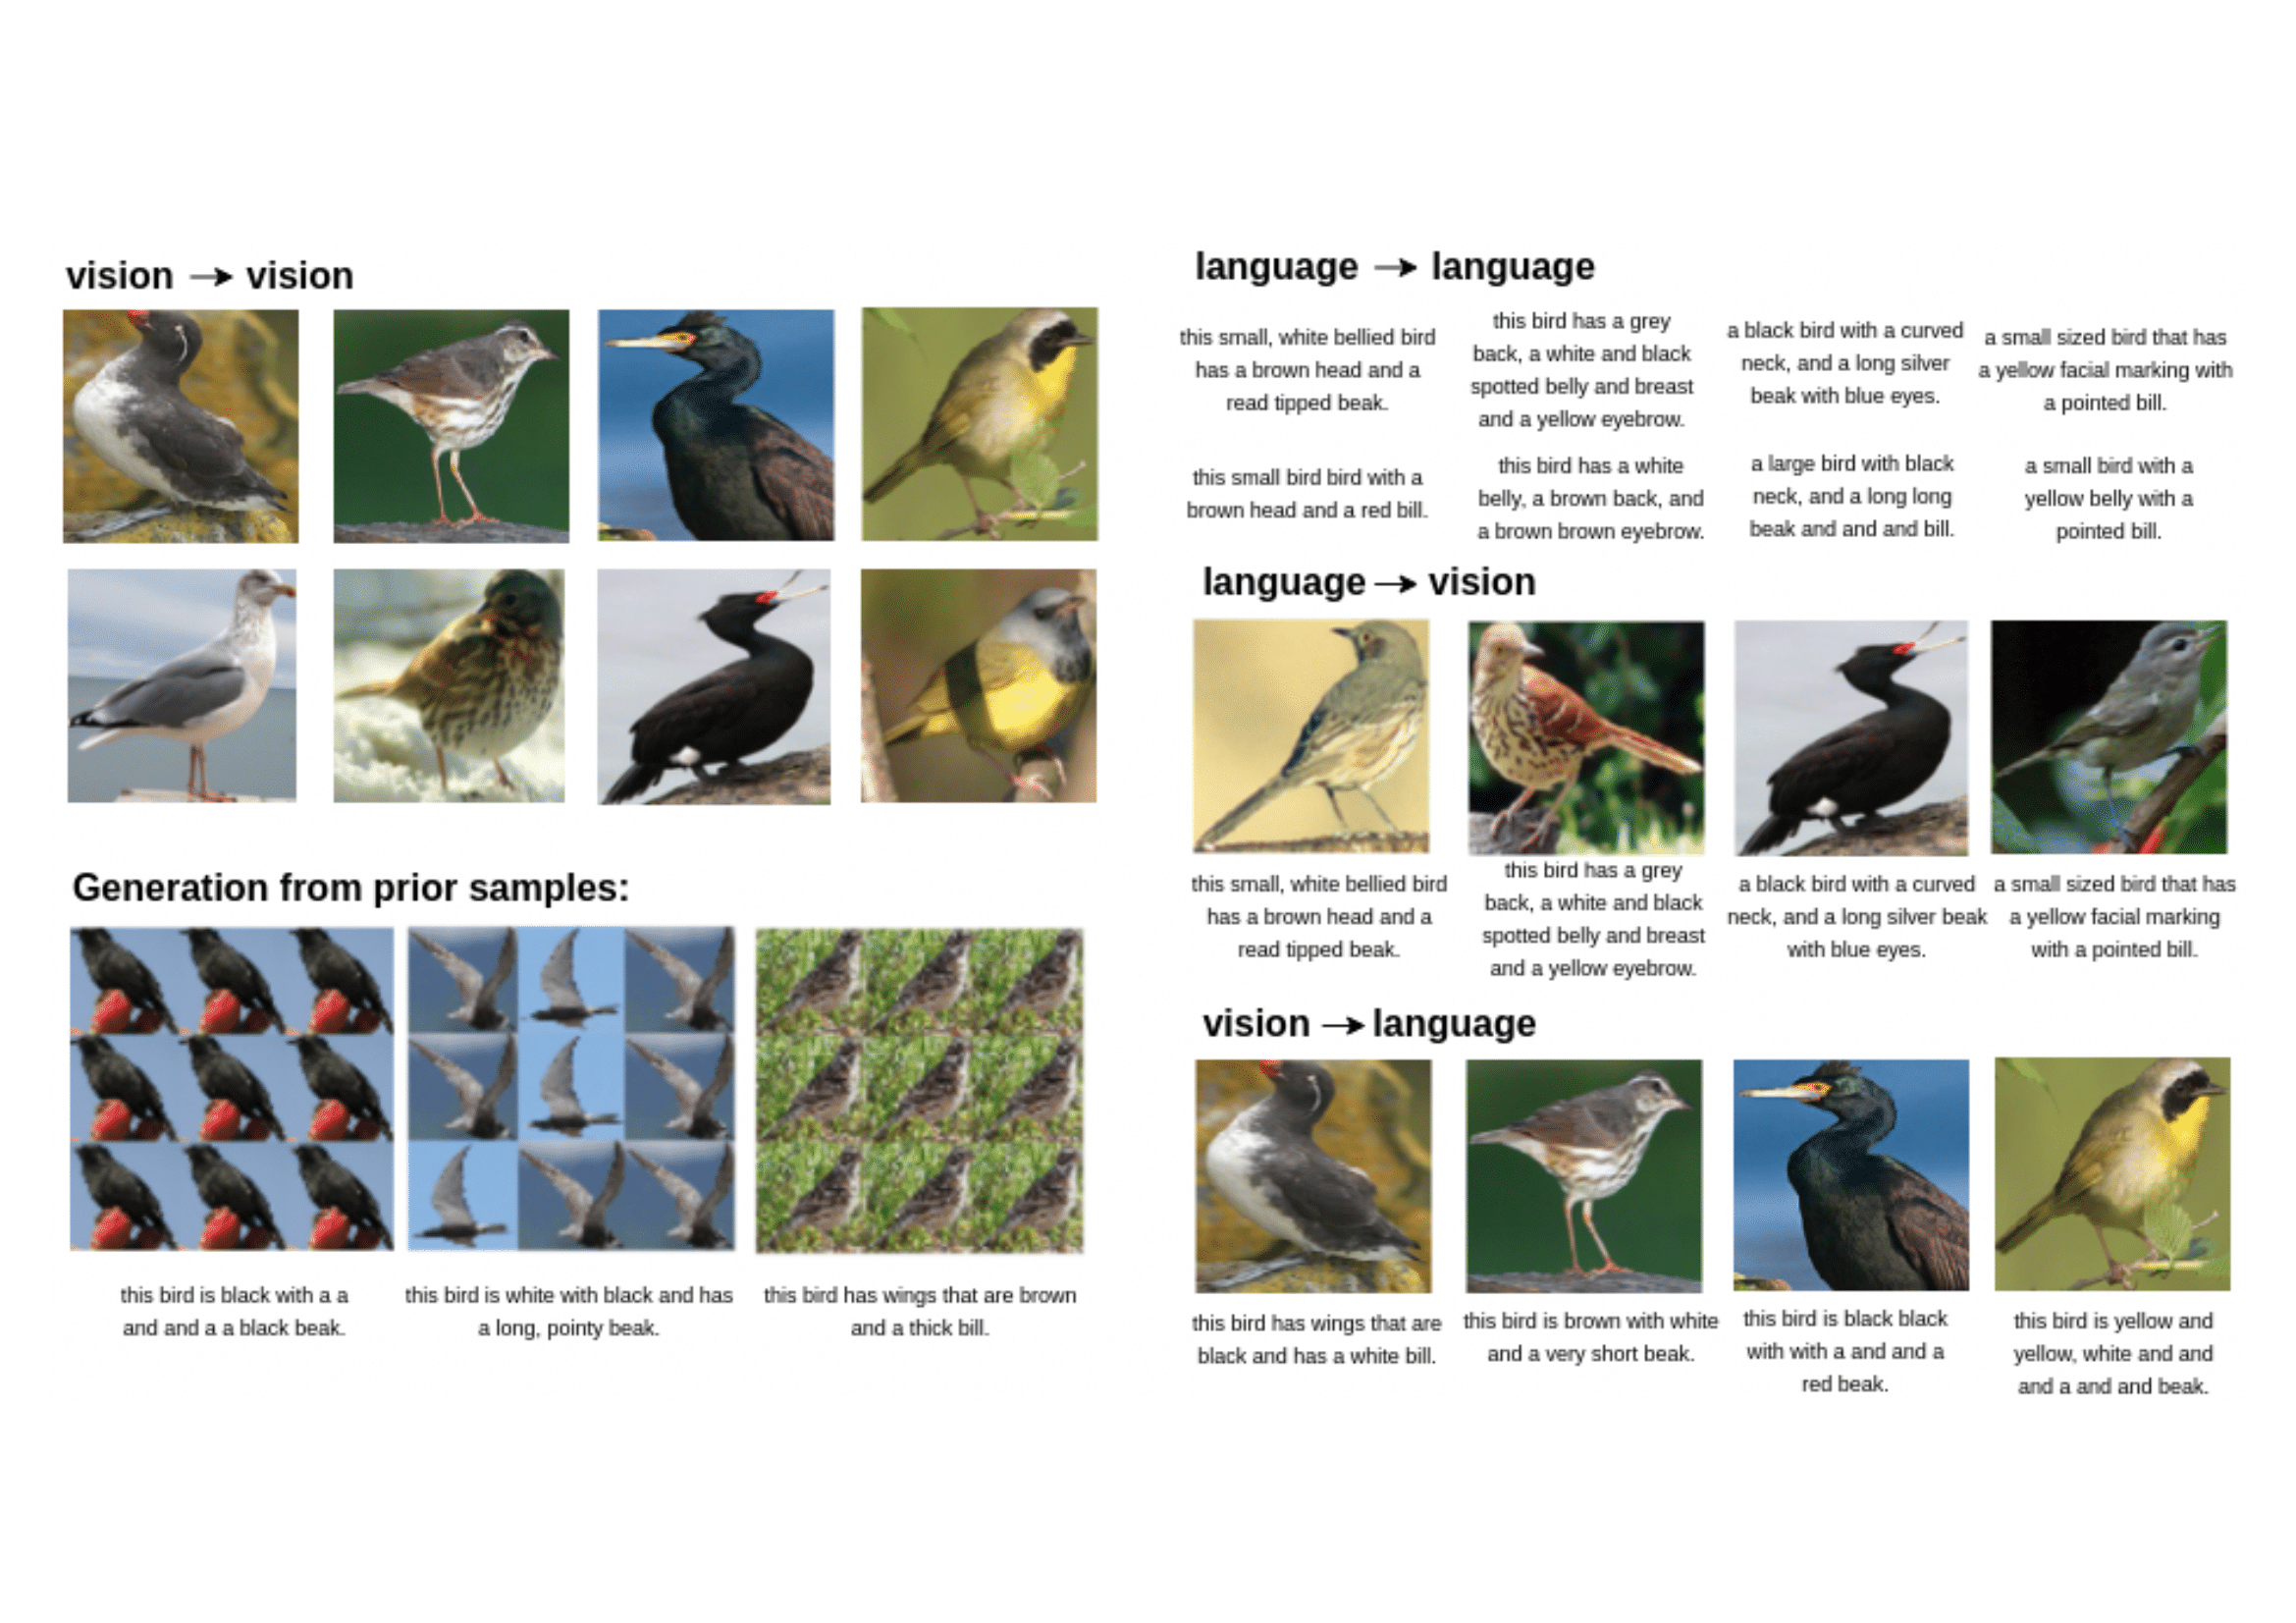
\includegraphics[scale=0.35]{birds.png}
        \caption{Qualitative results on CUB dataset.}
        \label{fig:birds}
    \end{figure}
\end{frame}


\begin{frame}{Literature}
    \begin{enumerate}
        \item \textbf{Main article} \href{https://proceedings.neurips.cc/paper/2019/file/0ae775a8cb3b499ad1fca944e6f5c836-Paper.pdf}
        {Variational Mixture-of-Experts Autoencoders for Multi-Modal Deep Generative Models}.
    \end{enumerate}
\end{frame}



\end{document}